% Method schematic (Figure 1 of the arXiv paper). Build: pdflatex schematic.tex
\documentclass[tikz,border=2pt]{standalone}
\usepackage[T1]{fontenc}
\usepackage{lmodern}
\usepackage{amsmath,amssymb}
\usetikzlibrary{arrows.meta,positioning,calc,fit,backgrounds,decorations.pathreplacing}

\definecolor{ink}{HTML}{1A1A19}
\definecolor{ink2}{HTML}{52514E}
\definecolor{muted}{HTML}{9A998F}
\definecolor{gridc}{HTML}{E4E3DE}
\definecolor{jblue}{HTML}{2A78D6}
\definecolor{lorange}{HTML}{EB6834}
\definecolor{violet}{HTML}{6250D6}
\definecolor{paper}{HTML}{F6F5F1}
\definecolor{bluebg}{HTML}{EEF4FC}

\tikzset{
  >={Stealth[length=4pt,width=3.2pt]},
  res/.style={circle,draw=ink2,line width=0.5pt,fill=white,minimum size=13pt,inner sep=0pt,font=\scriptsize},
  src/.style={res,draw=ink,fill=ink,text=white},
  box/.style={rectangle,rounded corners=2pt,draw=ink2,line width=0.5pt,fill=white,
              minimum height=15pt,inner sep=3pt,font=\footnotesize,align=center},
  ebox/.style={box,minimum width=17pt,minimum height=13pt,inner sep=1pt,font=\scriptsize},
  lab/.style={font=\footnotesize,text=ink},
  note/.style={font=\scriptsize,text=ink2,align=center},
  self/.style={->,line width=0.8pt,draw=lorange},
  bcast/.style={->,line width=0.8pt,draw=jblue},
  flow/.style={->,line width=0.6pt,draw=ink2},
}

\begin{document}
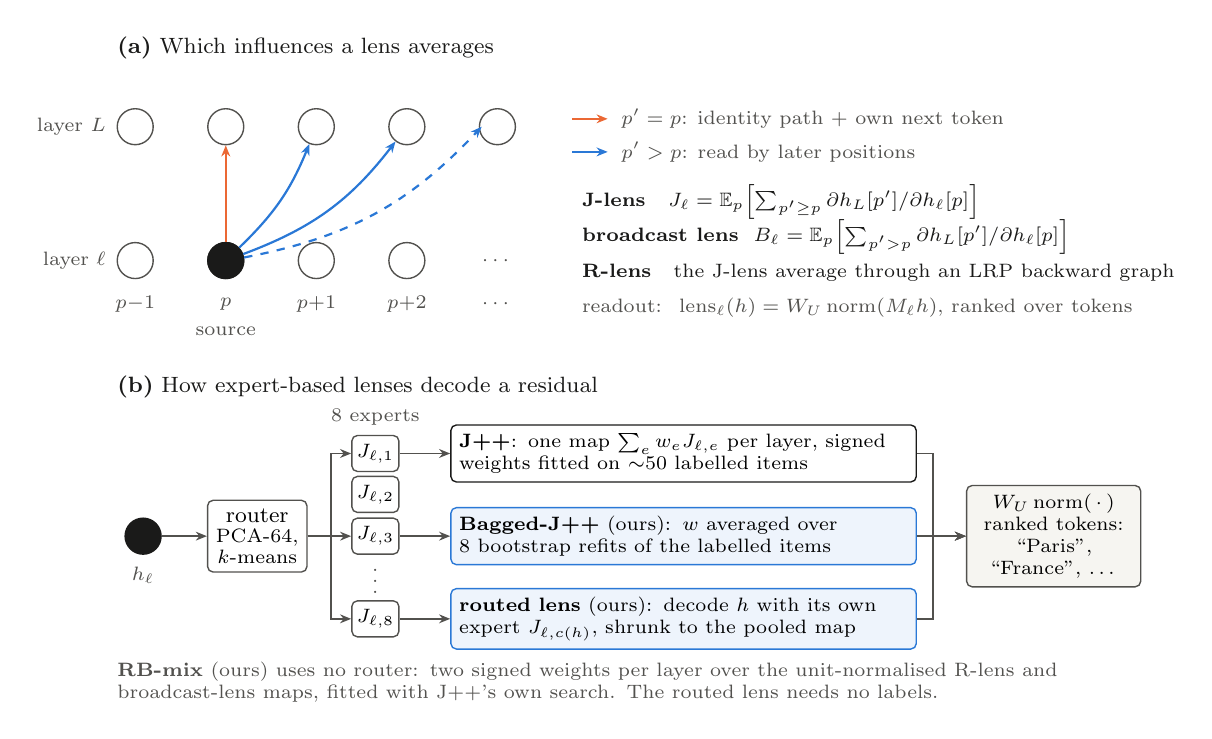
\begin{tikzpicture}[font=\footnotesize]

% ===================================================== panel (a): what the lens averages
\node[lab,anchor=west] at (-0.35,3.25) {\textbf{(a)} Which influences a lens averages};

% layer rows
\foreach \i/\name in {0/{p{-}1},1/p,2/{p{+}1},3/{p{+}2},4/{\cdots}} {
  \node[res] (top\i) at (1.15*\i,2.25) {};
  \node[note] at (1.15*\i,0.0) {$\name$};
}
\foreach \i in {0,1,2,3} { \node[res] (bot\i) at (1.15*\i,0.55) {}; }
\node[note] (botd) at (1.15*4,0.55) {$\cdots$};
\node[note] (topd) at (1.15*4,2.25) {};
\node[src] (bot1) at (1.15,0.55) {};
\node[note,anchor=east] at (-0.25,0.55) {layer $\ell$};
\node[note,anchor=east] at (-0.25,2.25) {layer $L$};
\node[note] at (1.15*1,-0.35) {source};

% influences
\draw[self] (bot1) -- (top1);
\draw[bcast] (bot1) to[bend right=12] (top2);
\draw[bcast] (bot1) to[bend right=16] (top3);
\draw[bcast,dashed] (bot1) to[bend right=18] ($(top3)+(0.95,0)$);

% legend / definitions
\begin{scope}[shift={(5.55,2.35)}]
  \draw[self] (0,0) -- (0.45,0); \node[note,anchor=west] at (0.5,0) {$p'=p$: identity path + own next token};
  \draw[bcast] (0,-0.42) -- (0.45,-0.42); \node[note,anchor=west] at (0.5,-0.42) {$p'>p$: read by later positions};
  \node[anchor=west,align=left,font=\scriptsize,text=ink] at (0,-1.05)
    {\textbf{J-lens} \ \ $J_\ell=\mathbb{E}_p\!\left[\sum_{p'\ge p}\partial h_L[p']/\partial h_\ell[p]\right]$};
  \node[anchor=west,align=left,font=\scriptsize,text=ink] at (0,-1.5)
    {\textbf{broadcast lens} \ $B_\ell=\mathbb{E}_p\!\left[\sum_{p'>p}\partial h_L[p']/\partial h_\ell[p]\right]$};
  \node[anchor=west,align=left,font=\scriptsize,text=ink] at (0,-1.95)
    {\textbf{R-lens} \ \ the J-lens average through an LRP backward graph};
  \node[anchor=west,align=left,font=\scriptsize,text=ink2] at (0,-2.4)
    {readout: \ $\mathrm{lens}_\ell(h)=W_U\,\mathrm{norm}(M_\ell h)$, ranked over tokens};
\end{scope}

% ===================================================== panel (b): expert-based lenses
\node[lab,anchor=west] at (-0.35,-1.05) {\textbf{(b)} How expert-based lenses decode a residual};

\node[res,fill=ink,draw=ink] (h) at (0.1,-2.95) {};
\node[note,below=1pt of h] {$h_\ell$};
\node[box] (router) at (1.55,-2.95) {router\\[-2pt]{\scriptsize PCA-64,}\\[-2pt]{\scriptsize $k$-means}};
\foreach \e/\yy in {1/-1.9,2/-2.42} { \node[ebox] (e\e) at (3.05,\yy) {$J_{\ell,\e}$}; }
\node[ebox] (e3) at (3.05,-2.95) {$J_{\ell,3}$};
\node[note] at (3.05,-3.42) {$\vdots$};
\node[ebox] (e8) at (3.05,-4.0) {$J_{\ell,8}$};
\node[note,anchor=south] at (3.05,-1.67) {8 experts};
\draw[flow] (h) -- (router);
\draw[flow] (router.east) -- ++(0.3,0) |- (e1.west);
\draw[flow] (router.east) -- (e3.west);
\draw[flow] (router.east) -- ++(0.3,0) |- (e8.west);

\tikzset{dec/.style={box,anchor=west,text width=5.7cm,align=left,font=\scriptsize,minimum height=0.62cm}}
\node[dec,draw=ink] (jpp) at (4.0,-1.9)
  {\textbf{J++}: one map $\sum_e w_e J_{\ell,e}$ per layer, signed\\ weights fitted on $\sim$50 labelled items};
\node[dec,draw=jblue,fill=bluebg] (bag) at (4.0,-2.95)
  {\textbf{Bagged-J++} (ours): $w$ averaged over\\ 8 bootstrap refits of the labelled items};
\node[dec,draw=jblue,fill=bluebg] (rout) at (4.0,-4.0)
  {\textbf{routed lens} (ours): decode $h$ with its own\\ expert $J_{\ell,c(h)}$, shrunk to the pooled map};
\draw[flow] (e1.east) -- (jpp.west);
\draw[flow] (e3.east) -- (bag.west);
\draw[flow] (e8.east) -- (rout.west);

\node[box,anchor=west,fill=paper,text width=2.0cm,font=\scriptsize] (out) at (10.55,-2.95)
  {$W_U\,\mathrm{norm}(\,\cdot\,)$\\ ranked tokens:\\ ``Paris'', ``France'', \dots};
\draw[flow] (jpp.east) -- ++(0.2,0) |- (out.west);
\draw[flow] (bag.east) -- (out.west);
\draw[flow] (rout.east) -- ++(0.2,0) |- (out.west);

\node[note,anchor=west,text width=13.0cm,align=left] at (-0.35,-4.8)
  {\textbf{RB-mix} (ours) uses no router: two signed weights per layer over the unit-normalised R-lens and
   broadcast-lens maps, fitted with J++'s own search. The routed lens needs no labels.};

\end{tikzpicture}
\end{document}
